%\section{Project Logic}
\chapter{Project Logic}
\label{chap:logic}
%\pagenumbering{arabic}

The reasoning in this work started by considering the characters of a problem that is recognizable in a Farm parallel pattern.
Then the study moved to consider how a GPU works, main architectural characteristics and facing its data parallel nature.
Next we had to think how to "merge" two such different behaviors, in order to reach reasonable performances \footnote{About expected performances see \hyperref[sect:overallLogic]{Section 3.3} and \hyperref[sect:tunings]{Section 3.4} for more clarifications}, i.e. almost competitive with a classic data parallel problem.
Finally, once the main idea behind the development was clear, we had to make some tunings.
All of these steps will be shown in detail in next sections.

\section{Streaming Parallelism: Farm pattern}
Stream parallel patterns describe problems exploiting parallelism among computations relative to
different, independent data items appearing on the program input stream.
Each independent computation end with the delivery of one single item on the program output stream.\\
We focused on farm pattern, modeling embarrassingly parallel stream parallelism. 
For example, consider the correspondent skeleton:\\
\texttt{let rec farm f =\\
	function\\
	EmptyStream -> EmptyStream\\
	| Stream(x,y) -> Stream((f x),(farm f y));;\\
	}
	
whose type is\\
\( farm :: (\alpha \rightarrow \beta) \rightarrow \alpha stream \rightarrow \beta stream \)\\

\textit{The parallel semantics, associated to the higher order functions, states that the computation of any items appearing on the input stream is performed in parallel}\\

In the farm case, according to the parallel semantics a number of parallel agents computing function \(f\) onto input data items equal to the number of items appearing onto the input stream could be used. This is not realistic, however, for two different reasons:

\begin{enumerate}
	\item items in the stream do not exist all at the same time. A stream is not a vector.
	Items of the stream may appear at different times. Actually, when we talk of consecutive items \(x_{i}\) and \(x_{i+1}\) of the stream we refer to items appearing onto the stream at times \(t_{i}\) and \(t_{i+1}\) with \(t_{i} < t_{i+1}\). As a consequence, it makes no sense to have a distinct parallel agent for all the items of the input stream, as at any given time only a fraction of the input stream will be available.
	
	\item if we use an agent to compute item \(x_{k}\), presumably the computation will end at some
	time \(t_{k}\). If item \(x_{j}\) appears onto the input stream at a time \(t_{j} < t_{k}\) this same agent
	can be used to compute item \(x_{j}\) rather than picking up a new agent. \\
\end{enumerate}
This is why the parallelism degree of a task farm is a critical parameter: a small parallelism degree doesn't exploit all the parallelism available (thus limiting the speedup), while a large parallelism degree may lead to inefficiencies as part of the parallel agents will be probably idle most of time \cite{spm}.\\

%In some skeleton frameworks, therefore, the parallelism degree is given as a parameter of
%the skeleton. The task farm skeleton is therefore defined as an high order function having
%(also) an integer as a parameter. This parameter represent their intended parallelism degree
%of the implementation of the skeleton. 
%However it has no effect on the “function” computed by the skeleton. It has only effect on the “parallel semantics” metadata.
%A task farm skeleton with a parallelism degree parameter may therefore be defined with
%the high order function
%let rec farm f n:int =
%function
%EmptyStream -> EmptyStream
%| Stream(x,y) -> Stream((f x),(farm f y));;
%whose type is now
%f arm :: (α → β) → int → α stream → β stream
%with the parallel semantics defined as follows:
%the computation of consecutive items of the input stream is performed in parallel on
%n parallel agents.
%These non functional parameters of skeletons generated quite a huge debate within the skeleton community. 
%On the one side, as skeletons pretend to abstract all the aspects related
%to parallelism exploitation, non functional parameters such as the parallelism degree should
%not be left under application programmer responsibility. Rather, they should be properly
%handled by the skeleton implementation, possibly being computed using some performance
%model of the skeleton (see Chap. 5). On the other side, such parameters can be used by
%expert programmers to express the fact they want to use exactly that amount of resources.
%As an example, they may want to experiment different parallelism degrees according to the
%type of the execution constrains of the applications. If the computation of the results is
%not urgent, smaller parallelism degrees may be required, whereas, in case of very urgent
%computations, higher parallelism degrees may be asked through non functional parameters.
%Consistently with the idea a skeleton is a programming abstraction hiding all the details
%related to parallelism exploitation pattern implementation, we agree on the idea that the
%better choice is to leave to the skeleton implementation the management of all the non
%functional skeleton parameters. In case the programmer is allowed to provide such kind of
%parameters, they will be only taken as loose requirements on the execution of the skeleton:
%the implementation of the skeleton will try to accommodate user requests, but in case
%the implementation could figure out the requests are not reasonable or that better choices
%could be made, these better choices will be actually taken and the user will be consequently
%informed.


%3.2.1
%Stream modelling
%An alternative way of defining stream parallel algorithmic skeletons assumes pipeline and
%farm just operate on a global input stream of data to produce a global stream of results. In
%this case, we may define pipelines and farms with much simpler higher order functions that
%do not operate on streams, actually, and then use these functions as parameters of another
%higher order function implementing stream parallelism. In this case, the pipeline skeleton
%will basically correspond to functional composition:
%let pipeline f g =
%function x -> (g (f x));;
%while task farm skeleton corresponds to identity:
%let farm f =
%function x -> (f x);;
%The higher order function taking care of exploiting parallelism can then be defined as follows:
%let rec streamer f x =
%match x with
%EmptyStream -> EmptyStream
%| Stream (v,s) -> Stream ((f v), (streamer f s));;
%such that, to define the filter/recognize program defined in Sec. 3.2 we can now write:
%let main =
%streamer (pipeline filter recognize);;
%Clearly, the parallel semantics associated to skeletons changes in this case, with respect
%to the parallel semantics we had when pipeline and farms actually processed streams. A
%parallel semantics is only associated to the streamer function as:
%the processing of independent input stream data items is performed in parallel
%whereas pipeline and farm have do not have associated any kind of parallel semantics.
%This way of modelling stream parallelism corresponds to the idea of structuring all stream
%parallel applications as farms 51 with more coarse grain computations as functional param-
%eter.
%Again, consider the filter/recognize example. Let’s suppose that the recognize phase is
%much more computationally expensive with respect to the filter phase. Using the explicit
%stream handling versions of pipeline and farm skeletons, we would write the program as
%let main =
%pipeline (filter) (farm recognize);;
%51 recall the parallel semantics previously given for the farm and look at the analogies in between the streamer
%function and the former definition of the farm higher order function58
%ALGORITHMIC SKELETONS
%Recalling the parallel semantics of these skeletons we can easily understand that given a
%stream with data items x 1 , . . . , x m (with x i appearing on the stream after x i−k for any k)
%the computations of
%recognize(y i ) recognize(y i+k )
%(being y i = f ilter(x i )) happen in parallel, as well as the computations of
%recognize(y i ) f ilter(x i+k )
%If we use the alternative modelling of stream parallelism described in this section, the
%program instead is written as
%let main =
%streamer (pipeline filter recognize);;
%and in this case the only computations happening in parallel are the
%recognize(f ilter(x i )) recognize(f ilter(x i+k ))


%3.3 A SIMPLE SKELETON FRAMEWORK
%Although different programming frameworks based on skeletons have been developed that
%sport each different algorithmic skeletons, a subset of common skeletons may be found in
%most of these frameworks. These common subset contains skeletons from three different
%classes of skeletons: stream parallel skeletons, data parallel skeletons and control parallel
%skeletons.
%3.3.1
%Stream parallel skeletons
%Stream parallel skeletons are those exploiting parallelism among computations relative to
%different, independent data items appearing on the program input stream. Each indepen-
%dent computation end with the delivery of one single item on the program output stream.
%Common stream parallel skeletons are the pipeline and task farm skeletons, whose definition
%in terms of higher order functions and parallel semantics has already been given in Sec. 3.2.
%The pipeline skeleton is typically used to model computations expressed in stages. In
%the general case, a pipeline may have more than two stages. The restriction to two stages
%as given by the definition in Sec. 3.3.4 guarantees strong typing and the ability to define
%pipelines with more than two stages as pipelines of pipelines. Given a stream of input tasks
%x m , . . . , x 1
%the pipeline with stages
%s 1 , . . . , s p
%computes the output stream
%s p (. . . s 2 (s 1 (x m )) . . .), . . . , s p (. . . s 2 (s 1 (x 1 )) . . .)
%The parallel semantics of the pipeline skeleton ensures all the stages will execute in
%parallel. In Chap. 5 we will see that this guarantees that the total time required to compute
%a single task (pipeline latency) is closed to the sum of the times required to compute the
%different stages. Also, it guarantees that the time needed to output a new result is close to
%time spent to compute a task by the longer stage in the pipeline.A SIMPLE SKELETON FRAMEWORK
%59
%The farm skeleton is used to model embarrassingly parallel computations, instead. The
%only functional parameter of a farm is the function f needed to compute the single task.
%Given a stream of input tasks
%x m , . . . , x 1
%the farm with function f computes the output stream
%f (x m ), . . . , f ( x 1 )



We recall that the only functional parameter of a farm is the function \(f\) needed to compute the single task.
Given a stream of input tasks
\begin{center}
	\(x_m , . . . , x_1\)\\
\end{center}
the farm with function \(f\) computes the output stream
\begin{center}
	\(f ( x_m ), . . . , f ( x_1 )\)\\
\end{center}
Its parallel semantics ensures it will process the single task in a time close to the time needed to compute \(f\) sequentially \cite{spm}. %The time between the delivery of two different task results, instead, can be made close to the time spent to compute f sequentially divided by the number of parallel agents used to execute the farm, i.e. its parallelism degree.
%\cite{spm}		


\section{CPU-GPGPU: heterogeneous architecture}
The target of this project was to exploit GPGPUs high parallelism to lighten the CPU from computation intensive problems, in particular associated to the above explained Farm parallel pattern.\\
So we asked ourselves what could happen if we wanted to manage such computations on streams in a way such that:
\begin{enumerate}
	\item Input stream arrives from host side, being directly generated by CPU or acquired from a remote source;
	
	\item Items are sent from host (main memory) to the GPU (global memory);
	
	\item GPU cores apply specific computations on all items of the stream (as soon as they available in global memory);
	
	\item Finally, computed elements will be copied back to host side and will become the output stream. \\
\end{enumerate}

	In this list our main concern is about data transfer, i.e. step 2 and 4. 
	Indeed these phases introduce an overhead per se, but especially in Farm parallel pattern they can be a not negligible bottleneck.\\
	We should not forget that our input is a stream: even if elements are available with a high throughput, they come "one by one".
	In reality, as we mentioned in the previous section, we have only a part of input available at one point, so it's not realistic to have one worker per stream element.
	
	In our case we can suppose Streaming Multiprocessors to be our Farm workers, so if we don't give enough work (items) to each core we would have a resources waste.\\
	Furthermore, we surely don't want to transfer from/to GPU one element at time but, at the same time, in some way we have to keep as much as possible the nature of a Stream parallel patterns.\\	
	Thus at this point has become necessary for first to find some stratagems:
	\begin{itemize}
		\item Hide as much as we can data transfer times, both in  \(Host \rightarrow Device\)  and  \(Device \rightarrow Host\)  direction;
		\item Exploit almost completely our workers resources, in other words try to make Streaming Multiprocessors as busy as possible.
	\end{itemize}

	
	\subsection{Overlapping: Data Transfer hiding}
	In \hyperref[subs:stream]{Section 2.3.3}, we introduced CUDA Streams and we recall that they can perform asynchronous memory copies to or from the GPU	concurrently with kernel execution. 
	Since the machines we worked on both have concurrency on data copy and kernel execution and they have 2 copy engines, we exploited this capability combined with streams.\\
	In this way we wanted to achieve a situation in which we could overlap, as much as it was possible, the time it took for the GPU to execute a kernel and the time it took to transfer data back and forth.
	
	As an example see Figure \ref{fig:threeStreams} to understand a simple case with 3 CUDA Streams.
	In that diagram we can see the expected behavior of three streams, but we can extend our expectations to more than three streams, without forgetting that we can have at most 2 data transfer at the same time (given that we've two copy engines).
	
	It's important to point out that not always we can have an ideal behavior in Streams, finding a performance improvement lower than the amount we expected.
	
	Overlap amount depends on several factors: on the order in which the commands are issued to each stream, whether or not the device supports overlap of data transfer and kernel execution, concurrent kernel execution, and/or concurrent data transfers, the balancing between data transfers time and kernel executions time.\\
	Given that our GPUs supported all kind of above mentioned concurrencies, among the above factors the only that can influence in our case are the order, in which commands are issued to each stream, and the kernel/data transfer time balancing.\\
	\begin{figure}
		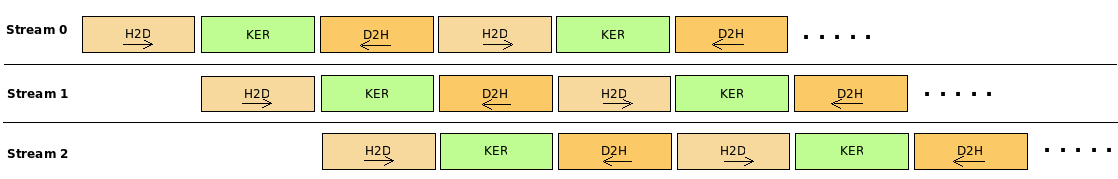
\includegraphics[width=\linewidth]{images/3Streams.png}
		\caption{Ideal behavior for 3 CUDA Streams.}
		\label{fig:threeStreams}
	\end{figure}
	We followed some useful guidelines to improve the potential for concurrent kernel execution:
	\begin{itemize}
		\item All independent operations should be issued before dependent operations;
		\item Synchronization of any kind should be delayed as long as possible.
	\end{itemize}

	For the former, we have that all operations are independent, given the Farm nature. Indeed all stream items and their computation given by workers, are independent.\\
	For the latter, we were careful to avoid \textit{Implicit synchronization}, this happens when are introduced host issued operations in-between different streams commands.\\
	Moreover we avoided all possible \textit{Explicit synchronizations} \footnote{In CUDA there are several command to force synchronization either between host and device, or between streams etc.}.
	
	Another important face of overlapping, is that we should try to balance Kernels work in such a way it's sufficient to hide the time spent in data transfers, as we quoted just above. 
	This said we can have two unfair scenarios:
	\begin{itemize}
		\item Data transfers take a small amount of time, while kernels are doing lot of computations;
		
		\item Data transfers take a big amount of time, with respect to time spent in kernel execution.
	\end{itemize}
	
	The former case may arise when we have heavy computations or \textit{"irregular kernels"}.
	By irregular we mean that any flow control instruction (\texttt{if}, \texttt{switch}, \texttt{do}, \texttt{for}, \texttt{while}) can significantly affect the instruction throughput by causing threads of the same warp to diverge; that is, to follow different execution paths.\\ 
	If this happens, the different execution paths must be serialized, increasing the total number of instructions executed for this warp. When all the different execution paths have completed, the threads converge back to the same execution path.	
	So we should avoid different execution paths within the same warp \cite{cudaguide}.\\
	% To obtain best performance in cases where the control flow depends on the thread ID, the controlling condition should be written so as to minimize the number of divergent warps. This is possible because the distribution of the warps across the block is deterministic
	% as mentioned in Section 4.1 of the CUDA C Programming Guide. A trivial example is when the controlling condition depends only on(threadIdx / WSIZE) where WSIZEis the warp size. In this case, no warp diverges because the controlling condition is perfectly aligned with the warps 
	
	
	Whilst the latter case can happen when we move an amount of data at each transfer such that it takes more time than calculations. So in this case the dominant factor will be the data transfer.	
	%So about these two scenarios we had to make some assumptions and tunings, that we will see in ********. 

	
	\subsection{Occupancy of GPU cores}
	Once we carried out the stream logic, we had to understand how to try to exploit almost every Streaming Multiprocessor at any given time.
	This means that we wanted to launch as many kernels as needed to arrive near the full \textit{\textbf{Occupancy}}.
	
	Clearly, when we start, we'll have a portion of time, a sort of "warm up" phase, where we'll have first data transfers and kernels. So we'll have a narrowed number of running kernels. 
	But as soon as we could have enough data transfers and so a lot of kernels, we would reach a workload peak on GPU.\\
	In practice, when we just said \textit{lot of kernels}, we meant a lot of small groups of items on which apply our computations, in other words this small items groups will be assigned each to a thread block.\\ Let's spend a bit to explain better what Occupancy means.\\

	To \textit{\textbf{maximize utilization}} the application should be structured in a way that it exposes
	as much parallelism as possible and efficiently maps this parallelism to the various	components of the system to keep them busy most of the time.\\
	Here main ways to maximize utilization:
	\begin{enumerate}
			\item \textbf{Application Level}
			At a high level, the application should maximize parallel execution between the host, the
			devices, and the bus connecting the host to the devices, by using \textit{asynchronous functions} calls and streams;
			
			
			\item \textbf{Device Level}
			At a lower level, the application should maximize parallel execution between the multiprocessors of a device.
			Multiple kernels can execute concurrently on a device, so maximum utilization can also be achieved by using streams to enable enough kernels to execute concurrently;
			
			
			\item \textbf{Multiprocessor Level}
			At an even lower level, the application should maximize parallel execution between the	various functional units within a multiprocessor.
			In particular, \textit{a GPU multiprocessor relies on thread-level parallelism to maximize utilization of its functional units}. 
	\end{enumerate}
	
	From the above, it's clear that occupancy is directly linked to the number of resident warps. At every instruction issue time, a warp scheduler selects a warp that is ready to execute its next instruction, if any, and issues the instruction to the active threads of the warp.\\
	The number of clock cycles it takes for a warp to be ready to execute its next instruction is called the \textit{\textbf{latency}, and full utilization is achieved when all warp schedulers always have some instruction to issue for some warp at every clock cycle during that latency period, or in other words,	when latency is completely "hidden"}. 
	
	The most common reason a warp is not ready, to execute its next instruction, is that the instruction's input operands are not available yet.\\
	If all input operands are registers, latency is caused by register dependencies, i.e., some of the input operands are written by some previous instruction(s) whose execution has	not completed yet.\\ In the case of a back-to-back register dependency (i.e., some input
	operand is written by the previous instruction), the latency is equal to the execution time of the previous instruction and the warp schedulers must schedule instructions for different warps during that time.\\
	%Execution time varies depending on the instruction, but it is typically about 11 clock cycles for devices of compute capability 3.x, which translates to 44 warps for devices of compute capability 3.x (assuming that warps 	execute instructions with maximum throughput, otherwise fewer warps are needed).
	%This is also assuming enough instruction-level parallelism so that schedulers are always able to issue pairs of instructions for each warp.
	%If some input operand resides in off-chip memory, the latency is much higher: 200 to 400 clock cycles for devices of compute capability 3.x. 
	
	%The number of warps required to keep the warp schedulers busy during such high latency periods depends on the kernel code and its degree of instruction-level parallelism. In general, more warps are required if the ratio of the number of instructions with no off-chip memory operands 	(i.e., arithmetic instructions most of the time) to the number of instructions with off-chip 	memory operands is low (this ratio is commonly called the arithmetic intensity of the program). For example, assume this ratio is 30, also assume the latencies are 300 cycles on devices of compute capability 3.x. Then about 40 warps are required for devices of compute capability 3.x (with the same assumptions as in the previous paragraph).
	Another reason a warp is not ready, to execute its next instruction, is that it is waiting at some \textit{memory fence} (\textit{Memory Fence Functions}) or synchronization point.\\ A synchronization point can force the multiprocessor to idle as	more and more warps wait for other warps in the same block to complete execution of instructions.\\
	So, having multiple resident blocks per multiprocessor can help reduce idling in this case, as warps from different blocks do not need to wait for each other at synchronization points.
	
	The \textit{number of blocks and warps residing on each multiprocessor for a given kernel call depends on the execution configuration of the call} (grid and block dimensions), the memory resources of the multiprocessor, and the resource requirements of the kernel \cite{cudaguide}.\\
	Register and shared memory are others important Occupancy variables, but we didn't focused much on them as on execution configuration.\\
%	The number of registers used by a kernel can have a significant impact on the number	of resident warps. For example, for devices of compute capability 6.x, if a kernel uses 64 registers and each block has 512 threads and requires very little shared memory, then two blocks (i.e., 32 warps) can reside on the multiprocessor since they require 2x512x64 registers, which exactly matches the number of registers available on the multiprocessor. But as soon as the kernel uses one more register, only one block (i.e.,16 warps) can be resident since two blocks would require 2x512x65 registers, which are more registers than are available on the multiprocessor. Therefore, the compiler attempts to minimize register usage while keeping register spilling (see Device Memory Accesses)	and the number of instructions to a minimum. Register usage can be controlled using the maxrregcount compiler option or launch bounds as described in Launch Bounds.
%	Each double variable and each long long variable uses two registers.

At this point, we had to reason about how to maximize Occupancy in our Farm parallel pattern.\\
For first, we have to make some assumptions:
\begin{itemize}
	\item no shared memory was used;
	\item we took a really poor amount of registers, given the really simple nature of our example Kernels \footnote{We'll see what kind of kernels we used to test the farm parallel pattern, with some code slices in  \hyperref[chap:impl]{Chapter 4}.}.
\end{itemize}  
So we mainly had to put our attention on kernel Execution configuration and number of kernels launched, in order to try to maximize the number of active warps inside each Streaming Multiprocessor.

\subsection{Occupancy drawbacks}
Occupancy is a very important factor to take into account, but it's more important to be aware that \textbf{occupancy isn't the only factor to take care of}.\\
In other words, not always trying to achieve maximum occupancy is the best idea, in some cases lower occupancy gives even better performances.\\
That's why in this work we had to take into account of both sides of occupancy, this is another reason that led us to experiment and measure various settings and implementations.

It is common to recommend running more threads per Streaming Multiprocessor and/or running more threads per thread block; the motivation is that this is the only way to hide \textit{latencies}.\\
Indeed, common beliefs are: multithreading is the only way to hide latency on GPU; shared memory is as fast as registers. Those facts aren't always true.

Some studies demonstrated how was possible to hide arithmetic latency or to hide memory latency using fewer threads, leading to code that runs faster.
The \textit{Latency} is the time required to perform an operation, for arithmetic operations it takes \(\approx20\) cycles; for memory we have \(\approx400+\) cycles instead.\\
This, in particular, means that  we can' t start a dependent operation for these times, but they can be hidden by overlapping with other operations.

\begin{lstlisting}
	x= a + b; // takes about 20 cycles to execute
	y = a + c; // independent, can start anytime(stall)
	z= x+ d; // dependent, must wait for completion
\end{lstlisting}
So \textit{latency hiding} means to do other operations when waiting for latency, this will make code run faster (not faster than the peak). For example another way, than occupancy, to hide latency is \textit{Instruction Level Parallelism}.\\
%Fallacy:Increasing occupancy is the only way to improve latency hiding–No, increasing ILP is another way.
Furthermore another common belief is that occupancy is a metric of utilization, but, as we anticipate, it's only one of the contributing factors.

Another latency is memory-bounded, let's take an example:
\begin{lstlisting}
	__global__ void memcpy( float *dst, float *src){
		int block = blockIdx.x+ blockIdx.y* gridDim.x;
		int index = threadIdx.x+ block * blockDim.x;
		float a0 = src[index];
		dst[index] = a0;
	}
\end{lstlisting}
To hide memory latency, using even fewer threads, we can do more parallel work per thread:
\begin{lstlisting}
	__global__ void memcpy( float*dst, float*src){
		int iblock= blockIdx.x+ blockIdx.y* gridDim.x;
		int index = threadIdx.x+ 2 * iblock* blockDim.x;
		float a0 = src[index]; 
		//no latency stall
		float a1 = src[index+blockDim.x]; 
		//stall
		dst[index] = a0;
		dst[index+blockDim.x] = a1;
	}
\end{lstlisting}
Note: threads don't stall on memory access, they stall on data dependency instead.

Performances improve copying 4 or even 8 floats per thread, instead of copying one and run more blocks and allocate shared memory to control occupancy.\\
For example some common concepts\footnote{From CUDA Programming Guide.} on CUDA says:
\begin{itemize}
\item "In general, more warps are required if the ratio of the number of instructions with no off-chip memory operands (...) to the number of instructions with off-chip memory operands is low";  %()–No, we’ve seen 87% of memory peak with only 4 warps per SM in a memory intensive kernel. 
\item “In fact, for all threads of a warp, accessing the shared memory is as fast as accessing a register as long as there are no bank conflicts between the threads..” 
\end{itemize}
For the former there are studies that shows how a reduced quantity of warps gives good performances on memory intensive kernels.\\
For the latter, in reality, shared memory bandwidth is lower than register bandwidth, in fact we should use registers to run close to the peak.
But requiring more registers can result in having a low occupancy.\\
So, in many cases, this can be accomplished by computing multiple outputs per thread (see above example on multiple floats copy)\cite{loweroccupancy}.

\section{Overall Logic}
\label{sect:overallLogica}
We have an input stream of items, in our case we chose \texttt{floats}, we don't know how much they are and their arrival frequency.
What our project's doing, will be summarized in the following steps:
\begin{enumerate}
	\item As items start to arrive, we accumulate say \(k\) items at time in a buffer;
	\item As the buffer is full, on a certain stream say \texttt{streams[k]}, we send out that chunk of data to the device (GPU Global memory);
	\item Immediately after the data transfer call, we launch the kernel execution, with a certain Execution configuration. The kernel call will be placed to \texttt{streams[k]} as well;
	\item Once the kernel ends its computations, we copy back to host, on \texttt{streams[k]}, the chunk of manipulated data as output buffer;
	\item From the output buffer we'll send each item as output stream. 
\end{enumerate}

	\begin{figure}
		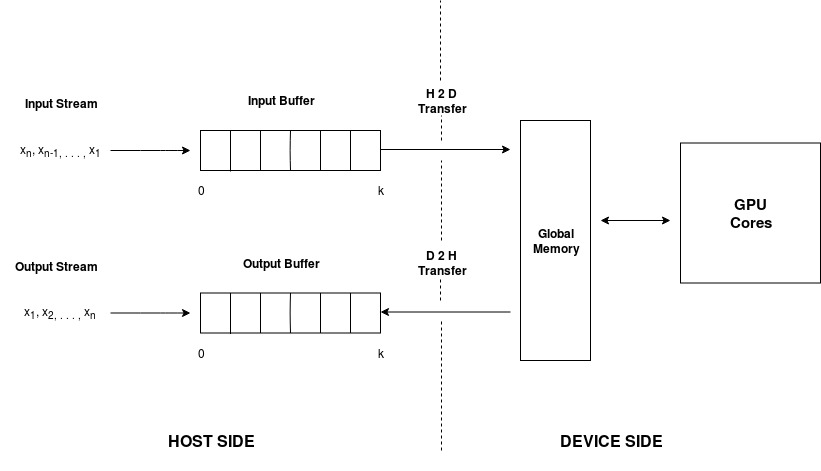
\includegraphics[width=\linewidth]{images/H2D.jpg}
		\caption{Here we have a general and broad graphical representation of our idea on how to fit a Farm parallel pattern on GPU architecture.}
		\label{fig:H2D}
	\end{figure}
	
	This behavior is illustrated graphically in Figure \ref{fig:H2D}. Here we can see our input stream and every \(k\) items we transfer them to Global memory of GPU.\\
	For reasons we showed in the previous sections, it would be unfeasible to work on single items but, at the same time, we should maintain a pattern as close as possible to Stream parallel. That's why we chose to work on chunks\footnote{We represented chunks as arrays, but they can be either small matrices or tiny images, as we'll see in \hyperref[chap:impl]{Chapter 4}.} of \(k\) items, where \(k\) is empirically determined to be a relatively small number of items and strictly related to execution configuration on kernel, in particular to block size.\\
	Items will be spread all over warps in a way such that for each item will be applied a set calculations, specified inside kernel code, that will be performed by one of the active threads in the warp.
	

	From that figure it may seems we're sending only \(k\) items at time to/from GPU, assuming \(k\) items in a buffer as a single item, this would correspond almost to a farm with one worker, processing one item per time. And this isn't completely what we wanted.\\
	\begin{figure}
		%	\hspace*{-2cm}  
		\vspace{-2cm}
		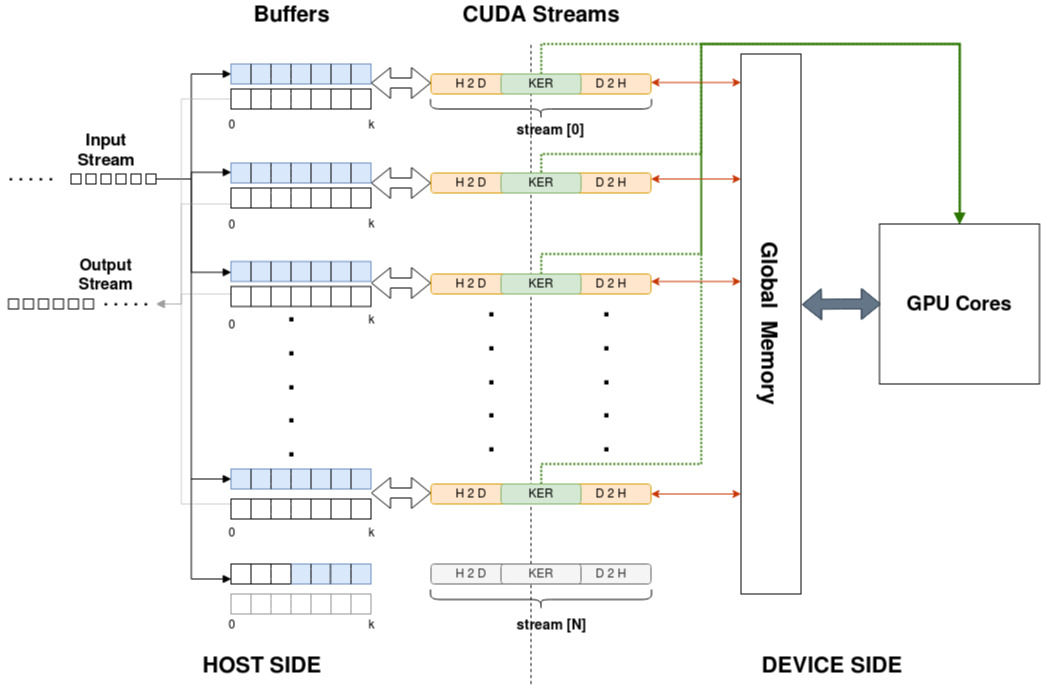
\includegraphics[scale=0.62,angle=-90]{images/overallLogic.jpg}
		\caption{Here we have a general and broad graphical representation of our idea on how to fit a Farm parallel pattern on GPU architecture.}
		\label{fig:overallLogic}
	\end{figure}
	So, here's where CUDA Streams \footnote{Don't confuse input/output stream in Farm parallel pattern with CUDA Streams.\\ These are two completely different notions: the first refers to the parallel pattern behavior of input/output data, the last refers to special CUDA commands (shown in \hyperref[subs:streams]{Section 2.3.3}).\\} come into play and we used them relying on the following ideas:
	\begin{enumerate}
		\item We have as many streams as Streaming Multiprocessors \footnote{Again CUDA Streams are a different concepts with respect to Streaming Multiprocessors. The first are a set of commands, the last are physical processing units.\\} and, at any given time, each of them hopefully issues a data transfer or a kernel executions;
		\item We should arrive at the point where each stream have issued at least one kernel launch, ideally we expect that each kernel execution is taken over by a certain multiprocessor. So we want to arrive at a moment in which we reach a work peak, where almost all SMs are busy;
		\item Obviously each kernel execution configuration should be well tuned, in order to take advantage of the maximum of resources in a multiprocessor. 
	\end{enumerate}
	

	All of those parameters have been established at first with some reasoning and assumptions on NVIDIA GPUs nature, later we moved on experimental proves \footnote{We'll see in next section more informations about Tunings.}. Measures and other estimation lead us to consider specific values for those variable parameters.\\
	So from the above facts is clear that we're trying to exploit each SM as a Farm parallel worker, furthermore, in such a way that all of those workers are as busy as possible. Note that our \textbf{SMs-workers} apply a \textbf{function-kernel} to all \textbf{tasks-chunks}.\\
	Bringing all pieces together we can summarize all project logic in Figure \ref{fig:overallLogic}.\\\\\\
	Putting down in words that schema:
				
		
	\begin{itemize}
		\item We have \(N\) CUDA streams, where \(N\) is the number of Streaming Multiprocessors in the machine were code is running;
		\item As input stream items arrive, we let them fill buffers;
		
		\item In a Round-Robin fashion we spread ready buffers all over the CUDA streams as follows:
		\begin{enumerate}
			\item As soon as the \(i^{th}\) buffer is full, it's asynchronously sent on \texttt{stream [i]} to the GPU, with the command \\ 
			\texttt{ \textbf{cudaMemcpyAsync}( devBuffer, hostBuffer, bytes, cudaMemcpyHostToDevice, \tab \tab \tab \tab stream [i]);}
			
			\item Soon after we put kernel call, on the \texttt{stream [i]}, to make desired computations on that buffer;
			
			\item Then, asynchronously again, we bring back results to host side, using the instruction \\
			\texttt{ cudaMemcpyAsync( devBuffer, hostBuffer, bytes, cudaMemcpyHostToDevice, \tab \tab \tab \tab stream[i]);}
			\item hopefully this should make a Streaming Multiprocessor,or a part, busy.
		\end{enumerate}
	\end{itemize}

	\begin{wrapfigure}[22]{r}{0.5\textwidth}
		%\begin{center}
		%\raggedleft
		\centering
		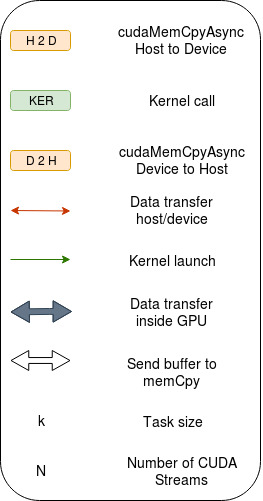
\includegraphics[width=1\linewidth]{images/logicLegenda.jpg}
		%\end{center}
		\caption{Legenda about Figure \ref{fig:overallLogic}.}
	\end{wrapfigure}
	Initially only few cores will be really busy, but as soon as the buffers and streams get full, the pressure on the GPU should increase, so we expected that workload should be enough to almost fill all of Streaming Multiprocessors.
	In particular, for us this means that we tried to have the maximum number possible of active threads inside each SM, having to do some work.\\
	Now let's put a magnifying glass upon Figure \ref{fig:overallLogic}, we want take a closer look to what we just said in Figure  \ref{fig:singleStream}.\\
	
	From that scheme, looking at violet numbered labels, we can see the order in which we issue commands in a stream, and this will be the order in which they will be issued to device side too, for that stream. \\
	The behavior of overlapping between different streams, isn't predictable. Anyway we should take advantage of the fact that, considering two different CUDA streams, we can overlap data transfer and/or kernel execution in a \texttt{stream [i]} with the ones in a \texttt{stream [k]} (for some \(k\in[0,N-1], \: for \: N =\# SMs\)). Obviously, when the number of streams is greater than 3, we can have only 2 data transfer operations issued at the same time (by two distinct streams) \footnote{As mentioned in \hyperref[chap:tools]{Chapter 2}, for concurrent memory copy between host and device, we have 2 copy engines.}.
	
	Note that in the Figure \ref{fig:singleStream}, we represented a single kernel execution as fully occupying an entire SM; in reality it's not exactly how it goes.
	We'll see how we practically tried out Streaming Multiprocessors \textit{occupancy} in  \hyperref[chap:experim]{Chapter 5}. \\
	
	So essentially if all of our reasoning and theories are right, we would expect that we can have an improvement, on completion time, roughly in the order of SMs number with respect to the \textit{classical approach}.\\
	By "classical approach" we mean to transfer data and execute kernels without any type of overlapping.\\ This is equivalent to send input to device, wait for data transfer completion on host, call kernel, send data back to host, only when all computations ended up, and finally results are transferred back to the host, waiting for data transfer ending.
	This similarly means that if, for example, we have 3 CUDA Stream we would expect to take an advantage on only at most 3 SMs (at peak work flow), so this should give us an improvement, in completion time, of at most 3 times compared to classical approach.\\

	\begin{figure}%[ht!]
		%	\hspace*{-2cm}  
		%\vspace{-2cm}
		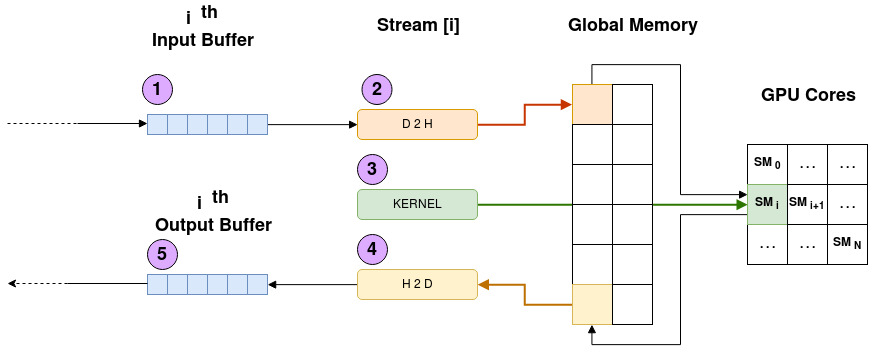
\includegraphics[scale=0.56]{images/singleStream.jpg}
		\caption{Here we can see what exactly happens in a certain CUDA Stream. Light violet numbered labels shows the order in which commands are issued by host to a certain stream.}
		\label{fig:singleStream}		
		
	\end{figure}	
\section{Tunings}
\label{sect:tunings}
	We showed a lot of peculiar behavior and architecture characteristics, because all of the above mentioned were taken into account for different implementation, tests datasets and results analysis.\\
	It's clear that, once we decided how to organize our Farm parallel pattern for the GPU, we had to give a huge work slice to experiments and empirical evaluations.
	This has many reasons why:
	\begin{itemize}
		\item It was important to think about a general logic, that wasn't architecture-dependent \footnote{At least we can say that the complexive view, showed in Fig. \ref{fig:overallLogic}, can be plausible with almost all NVIDIA architecture having >2 copy engines and allowing concurrent kernel execution. };
		
		\item To validate our total idea we had to make a lot of experiments, time measures, examples and even counterexamples;
		
		\item Clearly experiments required to get a little deeper on NVIDIA GPUs architecture, having a generic idea on good practices, not necessarily bounded to a specific model;
		
		\item Finally, we had to consider some feature totally model-bounded to launch tests and to give a sense to obtained results.
	\end{itemize}
	
	So after the logical phase, has followed a \textit{tuning phase}, that for first has been done facing general NVIDIA GPUs behavior and structure \footnote{In \hyperref[chap:experim]{Chapter 5} we'll mainly see tunings based on the GPUs used to run tests \textendash \textbf{P100} and \textbf{M40}.}.
	We followed for first some important best practices to try some good tunings:

	\begin{itemize}
		\item The effect of execution configuration on performance for a given kernel call generally
		depends on the kernel code, so experimentation is recommended and in fact we followed that approach;
		\item The number of threads per block should be chosen as a multiple of the warp size (generally equal to 32 threads) to avoid wasting computing resources with under-populated warps as much as possible \footnote{That's because kernels issue instructions in warps (groups of 32 threads). For example, if we have a block size of 50 threads, the GPU will still issue commands to 64 threads, so we would waste 14 of them idling.\\};
		\item We exploited \textbf{\textit{Occupancy Calculator}}\footnote{Those tools are included in CUDA Toolkit, they assist programmers in choosing thread block size based on kernel behavior, register and shared memory requirements.\\} both in spreadsheet and API functions\footnote{These are special function to call inside code, we'll see in \hyperref[chap:impl]{Chapter 4} a code example on how and where they are used.\\} formats , \cite{cudaguide}.
		 
	\end{itemize}

	Given those initial guidelines, it's important to highlight what are variable parameters in Figure \ref{fig:overallLogic}, on which the tuning was made:
	\begin{itemize}
		\item The number of Streams;		
		\item The number of blocks (grid size);
		\item The number of threads per block (block size) and as a consequence
		\item The buffer dimension.\\
	\end{itemize}
	After a lot of attempts and experiments, for each kernel type, we extrapolated best suitable values \footnote{Check \hyperref[chap:experim]{Chapter 5} to see all main values and their respective performances }.
 
			 
\subsection{Tuning on block and grid dimensions}
	It's important to understand some main concepts, that are the basis for the logic of this project.\\
	As we mentioned above, the variation on \textit{thread block size} and \textit{grid size}, can affect heavily performances, especially in an extreme scenario as the case study of this project.
	There's a tight bond in between \textit{Occupancy}, \textit{kernel execution configuration} and kernel code nature.
	For first note that a certain block, whatever its dimension is, will be run on a single Streaming Multiprocessor and once it's assigned it will never be moved; when resources are allocated for a thread block in an SM, it will become an \textit{active block}.\\
	In an SM we can have multiple blocks running independently, each of which grabbing its portion of resources, ie we can have multiple active blocks on a SM until they don't hit the maximum allowed.
	Here may emerge some particular cases:
	\begin{enumerate}
		\item Maximum block dimension (aka lot of threads per block), means that a smaller number of blocks, even only one, can fit in a certain SM;
		\item Small block dimension, means a higher number of blocks, even the maximum blocks number per SM supported, running on the same SM;
	\end{enumerate}
	
	In the first scenario, we can have cases of really good performances, but it may not be true when we have unbalanced workload for different blocks. This means that if a block has lot of work to do, it will monopolize resources of the SM in which it's running, making all other blocks, scheduled in the same SM, idle for too long (for example in our GPUs it may happens for \textit{blocksize = 1024}). 
	
	In the second scenario (for example for \textit{blocksize = 32}), we can have really poor performances due to poor resources exploitation, but for some kernels it may give a gain, especially in cases as the above mentioned of unbalanced workload.
	
	In general, there is a performance \textit{sweet spot} for middle values (for example usually identified in \textit{blocksize = 512}).\\
	%To better explain that concept, let's take a simple example. It's the first type of kernel we tested \footnote{We'll take a closer look on that case study, with implementation details, in \hyperref[chap:impl]{Chapter 4}.}, so suppose we have:
	%\begin{itemize}
	%	\item Vectors of floats as input and output;
	%	\item We have a "regular" kernel, in other words inside that we have not irregular workflows, we haven't divergent execution flowsand workload between all threads is almost the same;
	%	\item We avoid all types of synchronizations, both thread synchronization (\texttt{\_\_syncthreads()}) and host/device one (\texttt{cudaDeviceSynchronize()}).
	%\end{itemize}
	%In this situation
	So our tests had to face with the above explained behavior, without forgetting the nature of the various implemented kernels and the relative latencies.


\section{CPU/GPU Scheduling}
\label{sect:cpugpuscheduling}
In addition to the main logic of our project we introduced another branch of study.\\
In particular, we extended the Farm parallel pattern on GPGPU introducing a sort of \textit{\textbf{CPU/GPU Scheduler}}.\\
This consist in an implementation that, given an initial work percentage, it gradually and experimentally tunes those percentages to balance jobs.
In particular, the scheduler adjusts the dimensions of data chunks directed to CPU or GPU on the basis of previous measured completion times of both processors.\\
Clearly, starting from a user provided percentage, measured times are used to recompute percentages (and thus chunks dimension). So, in a finite number of algorithm steps, the two portion size will stabilize around two values.\\
This allow us to let host and device cooperate to apply same computations, but with different workloads. Clearly the main idea is to let GPU have a greater workload with respect to the one for CPU, so that  latter can be lighten from doing the entire computations; at the same time, having a good occupancy on GPU, we can gain a speedup compared to letting only one of the two processors doing all the work.\\

	
